Database testing is performed in a dynamic white-box manner. The tests are white-box as it is not the MySQL server we are testing, but that the database design
correspond to functionally that are expected.A total of 16 test cases have been designed, \autoref{fig:dbtest01-12} show the test design for test cases \#00 to \#11.
The identifier \code{TD0001} points to \autoref{fig:dbtd0001}, which explains each step to be performed for the test cases in \autoref{fig:dbtest01-12}.


\begin{figure}[H]
 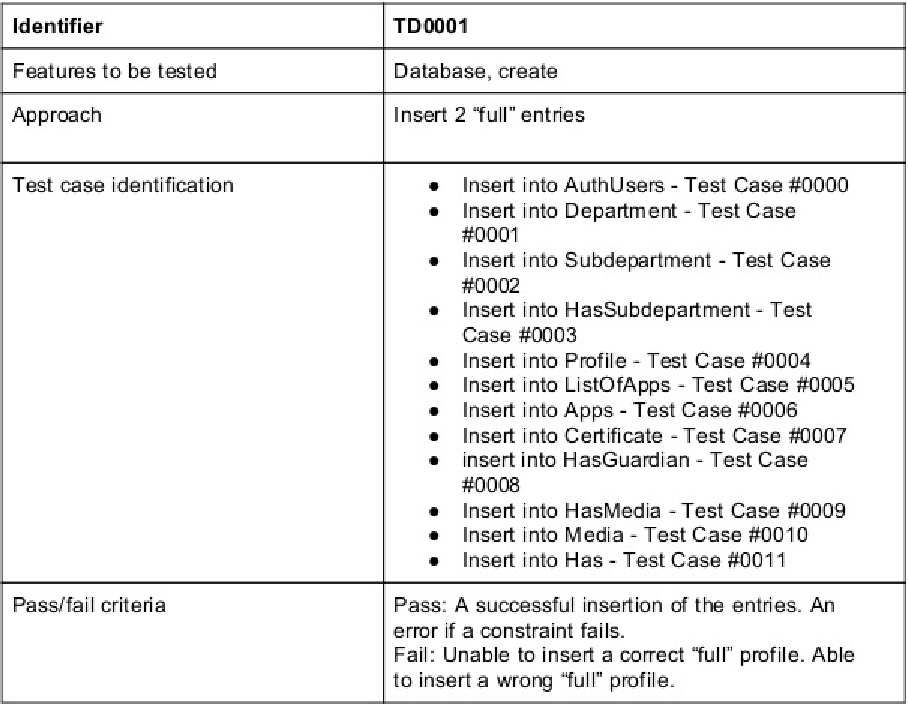
\includegraphics[scale=1.00]{images/dbtesttd0001}
 \caption{Testcase design of tests 01 to 12.}
  \label{fig:dbtest01-12}
\end{figure}

\begin{figure}[H]
 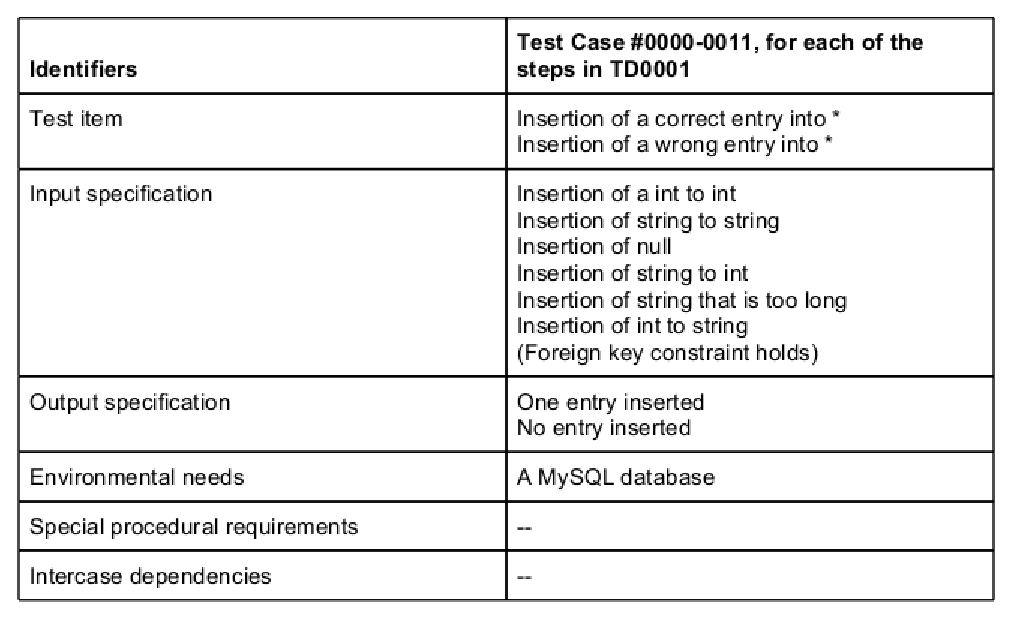
\includegraphics[scale=1.00]{images/dbtestcase01-12}
  \caption{Testcases 01 to 12}
  \label{fig:dbtd0001}
\end{figure}

All the database tests are done manually through a terminal and thus require human interpretation. \autoref{hej} shows an example of the test output, in this particular case attempting
to insert a user name longer than the allowed 45 characters. 


\begin{Code}
\begin{lstlisting}[label=hej,caption=Test case output]
--------------
INSERT INTO AuthUsers
values('tolongstring',null,1,
       'username00username00username00username00username00',
       'hansen')
--------------

ERROR 1406 (22001): Data too long for column 'username' at row 1
\end{lstlisting}
\end{Code}







